\section{Approach Upgrade}

	\begin{frame}
		\frametitle{NMPC with Switching Objective}
		\onslide<1->
		{
			\begin{block}{Optimization Problem}
				\parbox[c][3\baselineskip][t]{\textwidth}{
					\begin{align*}
					\underset{\vartheta^*,\mathbf{U}^*}{\text{min    }}
					J_{N_p}(\vartheta_k) = (1 - \tikzmark{a16}\beta_2 - \tikzmark{a17}\beta_3) \times J_1 + 
					\tikzmark{a18}\beta_2 \times J_2 - \tikzmark{a19}\beta_3 \times J_3
					\end{align*}
				}
			\end{block}
		}
		\onslide<3->
		{Objectives:}
		\begin{itemize}
			\onslide<4->
			{\item $J_1 = \ell_{p,1}(\cdot,\cdot)$}
			\onslide<5->
			{\item $J_2 = w_2 \times J_1 + J_4$}
			\onslide<6->
			{\item $J_3 = w_3 \times J_1 + J_5$ \\ [1cm]}
		\end{itemize}
		\onslide<7->
		{
			\[
			J_{N_p}(\vartheta_k) = 
			\begin{cases}
			\beta_2 = 0, \enspace \beta_3 = 1, 				& \text{if a dynaminc obstacle is detected} \\
			\beta_2 = 1, \enspace \beta_3 = 0, 				& \text{else, if the robot is near the goal} \\
			\beta_2 = 0, \enspace \beta_3 = 0, 				& \text{otherwise} 
			\end{cases}
			\]
		}
		\begin{tikzpicture}[overlay, remember picture]
		\coordinate (A16) at ($({pic cs:a16})+(1ex, 0.5ex)$);
		\coordinate (A17) at ($({pic cs:a17})+(1ex, 0.5ex)$);
		\coordinate (A18) at ($({pic cs:a18})+(1ex, 0.5ex)$);
		\coordinate (A19) at ($({pic cs:a19})+(1ex, 0.5ex)$);
		\onslide<2->{
			\node [fit=(A16), draw=tugreen, circle, thick, inner sep=4.5pt] (n16) {};
			\node [fit=(A17), draw=tugreen, circle, thick, inner sep=4.5pt] (n17) {};
			\node [fit=(A18), draw=tugreen, circle, thick, inner sep=4.5pt] (n18) {};
			\node [fit=(A19), draw=tugreen, circle, thick, inner sep=4.5pt] (n19) {};
			\node[overlay, below of= n16, node distance = 4em] at (8.5,5) (t16) {Binary};
			\node[overlay, below of= t16, node distance = 1em] (t16_1) {Multipliers};
			\draw [thick, -latex, tugreen] (n16.south) to [above] (t16.north);
			\draw [thick, -latex, tugreen] (n17.south) to [above] (t16.north);
			\draw [thick, -latex, tugreen] (n18.south) to [above] (t16.north);
			\draw [thick, -latex, tugreen] (n19.south) to [above] (t16.north);
		}
		\end{tikzpicture}
	\end{frame}
	
	\begin{frame}
		\frametitle{NMPC with Switching Objective Block Diagram}
		\begin{figure}[hbtp]
			\centering
			\includegraphics[scale=0.65]{pictures/block_diagram_polar_switch_1.pdf}
			\caption{NMPC Control Loop with Switching Objective}
		\end{figure}
	\end{frame}

	\begin{frame}
		\frametitle{Scenario \textrm{IV}: Dynamic Environment}
		\begin{figure}[hbtp]
			\centering
			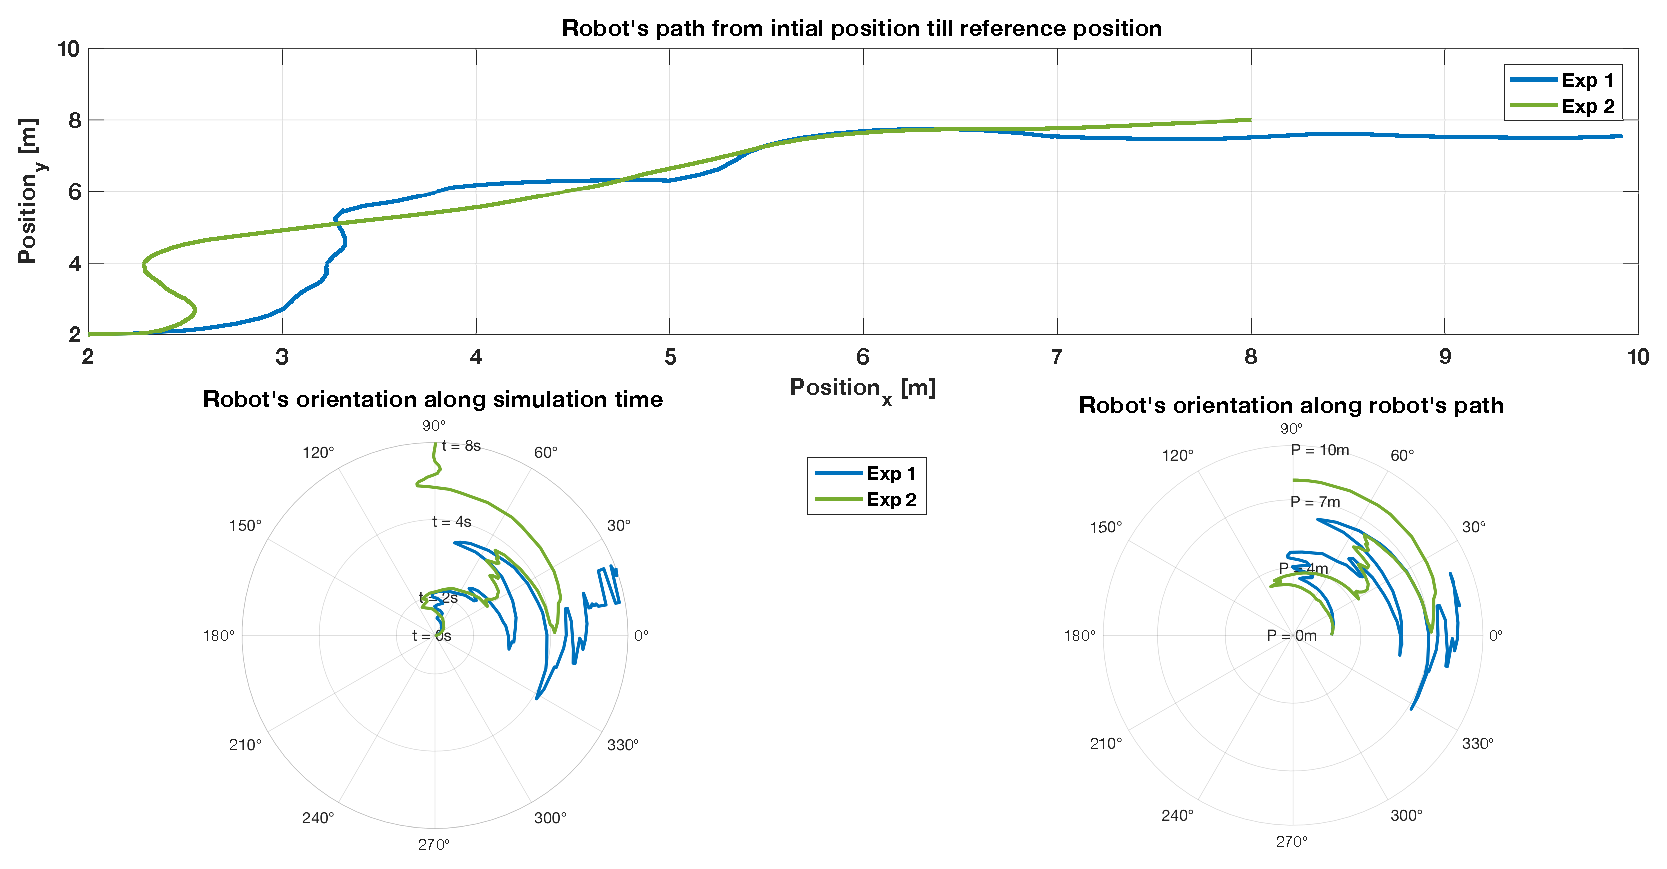
\includegraphics[scale=0.44]{pictures/graphs/sn3_states.eps}
			\caption{State Trajectory Evolution}
		\end{figure}
	\end{frame}
	
	\begin{frame}
		\frametitle{Scenario \textrm{IV}: Dynamic Environment}
		\begin{figure}[hbtp]
			\centering
			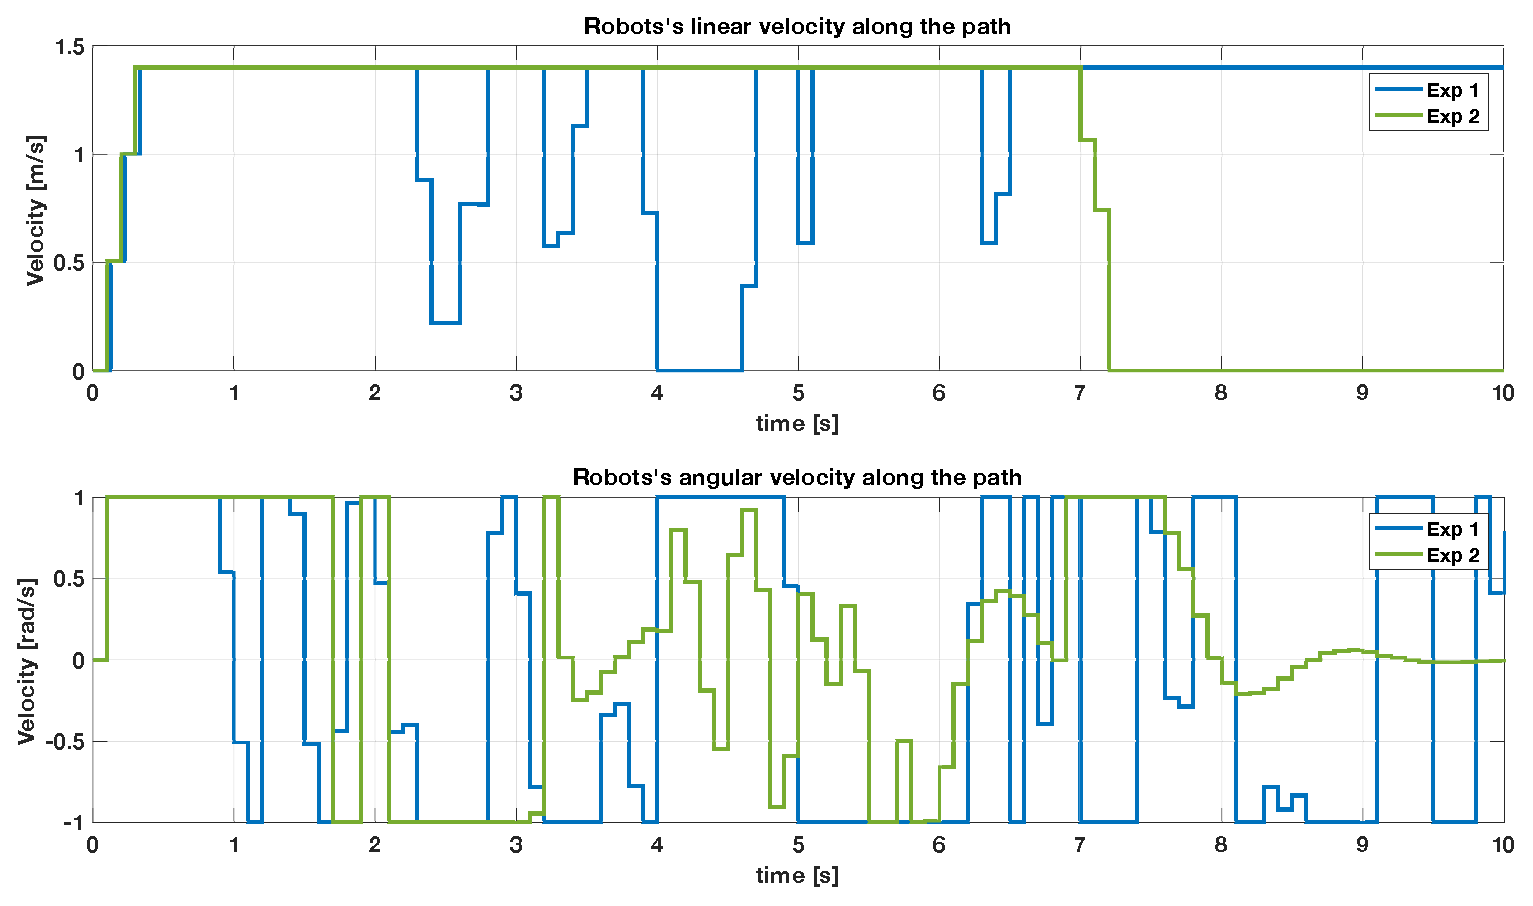
\includegraphics[scale=0.42]{pictures/graphs/sn3_inputs.eps}
			\caption{Input Trajectory Evolution}
		\end{figure}
	\end{frame}
	
	\begin{frame}
		\frametitle{Scenario \textrm{IV}: Dynamic Environment}
		\begin{figure}[hbtp]
			\centering
			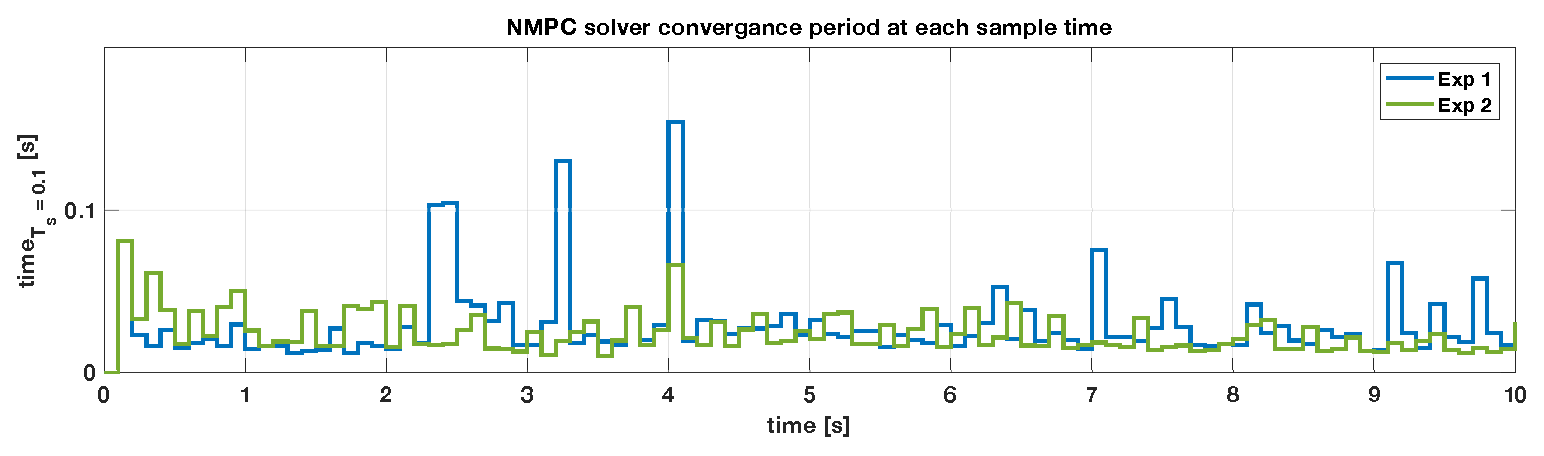
\includegraphics[scale=0.42]{pictures/graphs/sn3_solver_time.eps}
			\caption{NMPC Computational Effort}
		\end{figure}
	\end{frame}
	
	\begin{frame}
		\frametitle{Scenario \textrm{IV}: Dynamic Environment}
		\centering
		\movie[width=0.451\textwidth, height=0.865\textheight]
		{\includegraphics[width=0.45\textwidth]{pictures/good_1.png}}{videos/good_1.mov}
		\nocite{hoy_matveev_savkin_2015}
	\end{frame}